\chapter{Dry sand mining}
%\section{River bank instability due to sand mining}
%Much like the Paraná Guazú, sand mining is a relevant topic in the lower Mekong river. Previous studies have shown that incision due to the sand mining exists in this river and is of the order of 0.13 m per year \autocite{brunierRecentMorphologicalChanges2014}. \citeauthor{hackneyRiverBankInstability2020} showed that this river bed lowering not only has morphological consequences but also geotechnical ones, since a lower river bed can cause instability of the river banks.

%In the previous study it was found that, even in conservative scenarios, entire sections of river banks along the lower Mekong River would shift from a stable to a seasonally unstable condition. This means they are likely to fail during periods of heavy rainfall. In more extreme scenarios with more sand mining, the researchers found that 63\% of river banks would become seasonally unstable \autocite{hackneyIncreasedHydraulicRoughness2025}.

%In this chapter, the potential risks of river bank instability due to sand mining in the Paraná Guazú-river are investigated.

\section{Fracking in Argentina}
For much of its history, Argentina was regarded as a modest oil producer, struggling to meet its own energy demands. This perception shifted with the 2011 discovery of the Vaca Muerta shale formation, located in the Neuquén basin in Patagonia. The Argentine energy company YPF identified approximately 150 million barrels of recoverable oil in the field, which was regarded as a new source of hope for economic stability by the president \autocite{kraussArgentinaHopesBig2011}.

The discovery was followed by significant foreign investment from companies such as Total, ExxonMobil, Apache, and EOG Resources. More exploration was done and now it is clear that Argentina possesses the world’s fourth-largest shale oil and second-largest shale gas reserves. The Government of Argentina still views the oil and gas sector as a crucial part of its economy, by driving exports as well as generating foreign currency (ITA).

The Nuequén basin is located in the provinces of Neuquén, Mendoza, and Río Negro in the South of Argentina and has been an important basin for oil and gas since more than a century. Production started in 1918 and in 2004, 45\% of Argentinian oil production and 61\% of its gas production came from this area. This was done through conventional methods, but after the discovery of the Vaca Muerta shale basin, fracking has become increasingly important for the region and the country.

As can be seen in figure \ref{fig:oilgasprod}, oil production in Argentina has been steadily increasing since 2020, driven by increased production of the Vaca Muerta formations. After the exploration in 2010, oil from Vaca Muerto as a share of total Argentinian oil production has increased from virtually 0\% to 55\% today. Further, Vaca Muerta now accounts for 47\% of gas supply (PPT). Since Vaca Muerta is a shale reservoir, all oil and gas from this deposit is extracted by fracking.

\begin{figure}
    \centering
    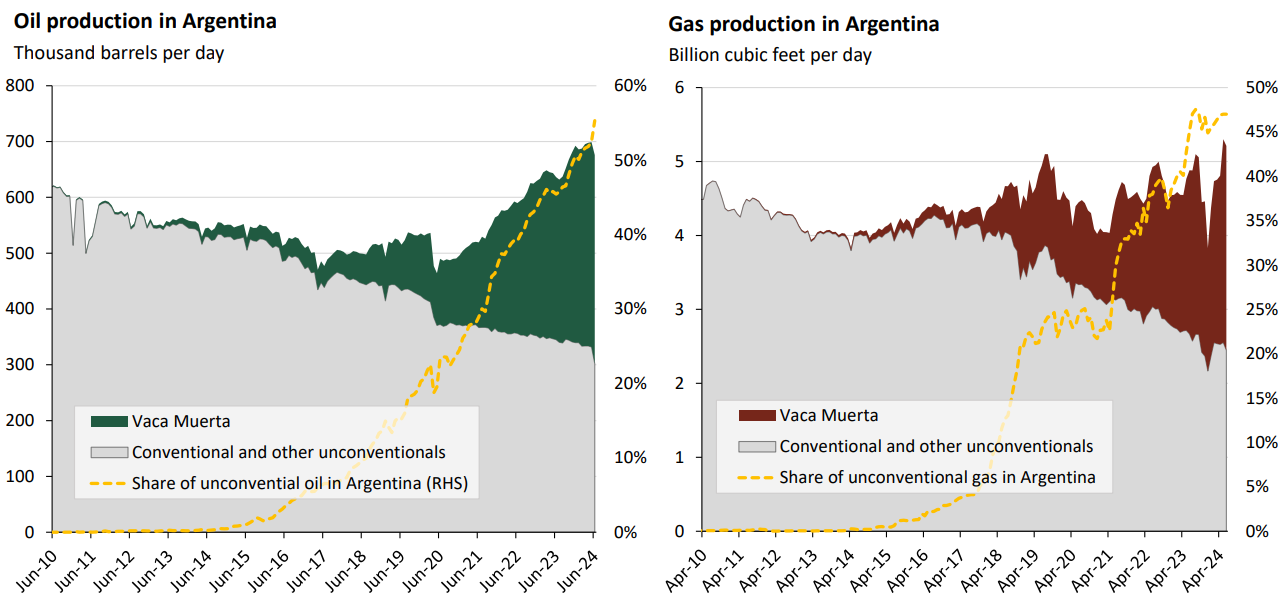
\includegraphics[width=1\linewidth]{figures/ch9/oilgasproduction.png}
    \caption{Oil and gas production in Argentina}
    \label{fig:oilgasprod}
\end{figure}

The numbers in \ref{fig:oilgasprod} help explain why fracking in the Neuquén basin is viewed as crucial to the development of Argentina's economy.



The stratigraphy of the Neuquen Basin is shown in Figure V-3. Of particular exploration
interest are the shales of the Middle Jurassic Los Molles and Late Jurassic-Early Cretaceous
Vaca Muerta formations. These two thick deepwater marine sequences sourced most of the oil
and gas fields in the basin and are considered the primary targets for shale gas development.

he Late Jurassic to Early Cretaceous (Tithonian-Berriasian) shale
of the Vaca Muerta Formation is considered the primary source rocks for conventional oil
production in the Neuquen Basin. The Vaca Muerta shale consists of finely-stratified black and
dark grey shale and lithographic lime-mudstone that totals 200 to 1,700 feet thick.10 The
organic-rich marine shale was deposited in reduced oxygen environment and contains Type II
kerogen. Although somewhat thinner than the Los Molles Fm, the Vaca Muerta shale has
higher TOC and is more widespread across the basin

The Vaca Muerta Formation thickens from the south and east towards the north and
west, ranging from absent to over 700 feet thick in the basin center.11 Depth ranges from
outcrop near the basin edges to over 9,000 feet deep in the central syncline.12

The Middle Jurassic (Toarcian-Aalenian) Los Molles Formation is
considered an important source rock for conventional oil and gas deposits in the Neuquen
Basin. Thermal maturity modeling indicates that hydrocarbon generation took place in the Los
Molles at 50 to 150 Ma, with the shallower Lajas Formation tight sands serving as reservoirs.3

The overlying Late Jurassic Aquilco Formation evaporites effectively seal this hydrocarbon
system, resulting in overpressuring (0.60 psi/ft) in parts of the basin.
The Los Molles shale is distributed across much of the Neuquen Basin, reaching more
than 3,300 ft thick in the central depocenter



The Vaca Muerta Formation has risked, technically recoverable shale gas and shale oil
resources of 308 Tcf of gas and 16 billion barrels of oil and condensate, from 1,202 Tcf and 270
billion barrels of risked, in-place shale gas and shale oil resources.

\section{Fracking practices}

\section{Fracking sand}




\section{Consequences of dry sand mining}

\section{Recommendations and mitigation strategies}